% Options for packages loaded elsewhere
\PassOptionsToPackage{unicode}{hyperref}
\PassOptionsToPackage{hyphens}{url}
\PassOptionsToPackage{dvipsnames,svgnames,x11names}{xcolor}
%
\documentclass[
  letterpaper,
  DIV=11,
  numbers=noendperiod]{scrartcl}

\usepackage{amsmath,amssymb}
\usepackage{iftex}
\ifPDFTeX
  \usepackage[T1]{fontenc}
  \usepackage[utf8]{inputenc}
  \usepackage{textcomp} % provide euro and other symbols
\else % if luatex or xetex
  \usepackage{unicode-math}
  \defaultfontfeatures{Scale=MatchLowercase}
  \defaultfontfeatures[\rmfamily]{Ligatures=TeX,Scale=1}
\fi
\usepackage{lmodern}
\ifPDFTeX\else  
    % xetex/luatex font selection
\fi
% Use upquote if available, for straight quotes in verbatim environments
\IfFileExists{upquote.sty}{\usepackage{upquote}}{}
\IfFileExists{microtype.sty}{% use microtype if available
  \usepackage[]{microtype}
  \UseMicrotypeSet[protrusion]{basicmath} % disable protrusion for tt fonts
}{}
\makeatletter
\@ifundefined{KOMAClassName}{% if non-KOMA class
  \IfFileExists{parskip.sty}{%
    \usepackage{parskip}
  }{% else
    \setlength{\parindent}{0pt}
    \setlength{\parskip}{6pt plus 2pt minus 1pt}}
}{% if KOMA class
  \KOMAoptions{parskip=half}}
\makeatother
\usepackage{xcolor}
\setlength{\emergencystretch}{3em} % prevent overfull lines
\setcounter{secnumdepth}{-\maxdimen} % remove section numbering
% Make \paragraph and \subparagraph free-standing
\makeatletter
\ifx\paragraph\undefined\else
  \let\oldparagraph\paragraph
  \renewcommand{\paragraph}{
    \@ifstar
      \xxxParagraphStar
      \xxxParagraphNoStar
  }
  \newcommand{\xxxParagraphStar}[1]{\oldparagraph*{#1}\mbox{}}
  \newcommand{\xxxParagraphNoStar}[1]{\oldparagraph{#1}\mbox{}}
\fi
\ifx\subparagraph\undefined\else
  \let\oldsubparagraph\subparagraph
  \renewcommand{\subparagraph}{
    \@ifstar
      \xxxSubParagraphStar
      \xxxSubParagraphNoStar
  }
  \newcommand{\xxxSubParagraphStar}[1]{\oldsubparagraph*{#1}\mbox{}}
  \newcommand{\xxxSubParagraphNoStar}[1]{\oldsubparagraph{#1}\mbox{}}
\fi
\makeatother

\usepackage{color}
\usepackage{fancyvrb}
\newcommand{\VerbBar}{|}
\newcommand{\VERB}{\Verb[commandchars=\\\{\}]}
\DefineVerbatimEnvironment{Highlighting}{Verbatim}{commandchars=\\\{\}}
% Add ',fontsize=\small' for more characters per line
\usepackage{framed}
\definecolor{shadecolor}{RGB}{241,243,245}
\newenvironment{Shaded}{\begin{snugshade}}{\end{snugshade}}
\newcommand{\AlertTok}[1]{\textcolor[rgb]{0.68,0.00,0.00}{#1}}
\newcommand{\AnnotationTok}[1]{\textcolor[rgb]{0.37,0.37,0.37}{#1}}
\newcommand{\AttributeTok}[1]{\textcolor[rgb]{0.40,0.45,0.13}{#1}}
\newcommand{\BaseNTok}[1]{\textcolor[rgb]{0.68,0.00,0.00}{#1}}
\newcommand{\BuiltInTok}[1]{\textcolor[rgb]{0.00,0.23,0.31}{#1}}
\newcommand{\CharTok}[1]{\textcolor[rgb]{0.13,0.47,0.30}{#1}}
\newcommand{\CommentTok}[1]{\textcolor[rgb]{0.37,0.37,0.37}{#1}}
\newcommand{\CommentVarTok}[1]{\textcolor[rgb]{0.37,0.37,0.37}{\textit{#1}}}
\newcommand{\ConstantTok}[1]{\textcolor[rgb]{0.56,0.35,0.01}{#1}}
\newcommand{\ControlFlowTok}[1]{\textcolor[rgb]{0.00,0.23,0.31}{\textbf{#1}}}
\newcommand{\DataTypeTok}[1]{\textcolor[rgb]{0.68,0.00,0.00}{#1}}
\newcommand{\DecValTok}[1]{\textcolor[rgb]{0.68,0.00,0.00}{#1}}
\newcommand{\DocumentationTok}[1]{\textcolor[rgb]{0.37,0.37,0.37}{\textit{#1}}}
\newcommand{\ErrorTok}[1]{\textcolor[rgb]{0.68,0.00,0.00}{#1}}
\newcommand{\ExtensionTok}[1]{\textcolor[rgb]{0.00,0.23,0.31}{#1}}
\newcommand{\FloatTok}[1]{\textcolor[rgb]{0.68,0.00,0.00}{#1}}
\newcommand{\FunctionTok}[1]{\textcolor[rgb]{0.28,0.35,0.67}{#1}}
\newcommand{\ImportTok}[1]{\textcolor[rgb]{0.00,0.46,0.62}{#1}}
\newcommand{\InformationTok}[1]{\textcolor[rgb]{0.37,0.37,0.37}{#1}}
\newcommand{\KeywordTok}[1]{\textcolor[rgb]{0.00,0.23,0.31}{\textbf{#1}}}
\newcommand{\NormalTok}[1]{\textcolor[rgb]{0.00,0.23,0.31}{#1}}
\newcommand{\OperatorTok}[1]{\textcolor[rgb]{0.37,0.37,0.37}{#1}}
\newcommand{\OtherTok}[1]{\textcolor[rgb]{0.00,0.23,0.31}{#1}}
\newcommand{\PreprocessorTok}[1]{\textcolor[rgb]{0.68,0.00,0.00}{#1}}
\newcommand{\RegionMarkerTok}[1]{\textcolor[rgb]{0.00,0.23,0.31}{#1}}
\newcommand{\SpecialCharTok}[1]{\textcolor[rgb]{0.37,0.37,0.37}{#1}}
\newcommand{\SpecialStringTok}[1]{\textcolor[rgb]{0.13,0.47,0.30}{#1}}
\newcommand{\StringTok}[1]{\textcolor[rgb]{0.13,0.47,0.30}{#1}}
\newcommand{\VariableTok}[1]{\textcolor[rgb]{0.07,0.07,0.07}{#1}}
\newcommand{\VerbatimStringTok}[1]{\textcolor[rgb]{0.13,0.47,0.30}{#1}}
\newcommand{\WarningTok}[1]{\textcolor[rgb]{0.37,0.37,0.37}{\textit{#1}}}

\providecommand{\tightlist}{%
  \setlength{\itemsep}{0pt}\setlength{\parskip}{0pt}}\usepackage{longtable,booktabs,array}
\usepackage{calc} % for calculating minipage widths
% Correct order of tables after \paragraph or \subparagraph
\usepackage{etoolbox}
\makeatletter
\patchcmd\longtable{\par}{\if@noskipsec\mbox{}\fi\par}{}{}
\makeatother
% Allow footnotes in longtable head/foot
\IfFileExists{footnotehyper.sty}{\usepackage{footnotehyper}}{\usepackage{footnote}}
\makesavenoteenv{longtable}
\usepackage{graphicx}
\makeatletter
\newsavebox\pandoc@box
\newcommand*\pandocbounded[1]{% scales image to fit in text height/width
  \sbox\pandoc@box{#1}%
  \Gscale@div\@tempa{\textheight}{\dimexpr\ht\pandoc@box+\dp\pandoc@box\relax}%
  \Gscale@div\@tempb{\linewidth}{\wd\pandoc@box}%
  \ifdim\@tempb\p@<\@tempa\p@\let\@tempa\@tempb\fi% select the smaller of both
  \ifdim\@tempa\p@<\p@\scalebox{\@tempa}{\usebox\pandoc@box}%
  \else\usebox{\pandoc@box}%
  \fi%
}
% Set default figure placement to htbp
\def\fps@figure{htbp}
\makeatother

\KOMAoption{captions}{tableheading}
\makeatletter
\@ifpackageloaded{caption}{}{\usepackage{caption}}
\AtBeginDocument{%
\ifdefined\contentsname
  \renewcommand*\contentsname{Table of contents}
\else
  \newcommand\contentsname{Table of contents}
\fi
\ifdefined\listfigurename
  \renewcommand*\listfigurename{List of Figures}
\else
  \newcommand\listfigurename{List of Figures}
\fi
\ifdefined\listtablename
  \renewcommand*\listtablename{List of Tables}
\else
  \newcommand\listtablename{List of Tables}
\fi
\ifdefined\figurename
  \renewcommand*\figurename{Figure}
\else
  \newcommand\figurename{Figure}
\fi
\ifdefined\tablename
  \renewcommand*\tablename{Table}
\else
  \newcommand\tablename{Table}
\fi
}
\@ifpackageloaded{float}{}{\usepackage{float}}
\floatstyle{ruled}
\@ifundefined{c@chapter}{\newfloat{codelisting}{h}{lop}}{\newfloat{codelisting}{h}{lop}[chapter]}
\floatname{codelisting}{Listing}
\newcommand*\listoflistings{\listof{codelisting}{List of Listings}}
\makeatother
\makeatletter
\makeatother
\makeatletter
\@ifpackageloaded{caption}{}{\usepackage{caption}}
\@ifpackageloaded{subcaption}{}{\usepackage{subcaption}}
\makeatother

\usepackage{bookmark}

\IfFileExists{xurl.sty}{\usepackage{xurl}}{} % add URL line breaks if available
\urlstyle{same} % disable monospaced font for URLs
\hypersetup{
  pdftitle={Analise\_Flood\_Sentinel},
  colorlinks=true,
  linkcolor={blue},
  filecolor={Maroon},
  citecolor={Blue},
  urlcolor={Blue},
  pdfcreator={LaTeX via pandoc}}


\title{Analise\_Flood\_Sentinel}
\author{}
\date{}

\begin{document}
\maketitle


\subsection{Análise Exploratória e Explanatória em R para o conjunto
``flood.csv''}\label{anuxe1lise-exploratuxf3ria-e-explanatuxf3ria-em-r-para-o-conjunto-flood.csv}

\subsection{Instalar pacotes}\label{instalar-pacotes}

\begin{verbatim}
Installing packages into 'C:/Users/JonasLuisdaSilva/AppData/Local/R/win-library/4.5'
(as 'lib' is unspecified)
\end{verbatim}

\begin{verbatim}
package 'tidyverse' successfully unpacked and MD5 sums checked
package 'GGally' successfully unpacked and MD5 sums checked
package 'corrplot' successfully unpacked and MD5 sums checked
package 'knitr' successfully unpacked and MD5 sums checked
package 'gridExtra' successfully unpacked and MD5 sums checked
package 'Metrics' successfully unpacked and MD5 sums checked

The downloaded binary packages are in
    C:\Users\JonasLuisdaSilva\AppData\Local\Temp\Rtmp6dfTM1\downloaded_packages
\end{verbatim}

Carregar as bibliotecas

\begin{Shaded}
\begin{Highlighting}[]
\FunctionTok{library}\NormalTok{(tidyverse)}
\end{Highlighting}
\end{Shaded}

\begin{verbatim}
-- Attaching core tidyverse packages ------------------------ tidyverse 2.0.0 --
v dplyr     1.1.4     v readr     2.1.5
v forcats   1.0.0     v stringr   1.5.1
v ggplot2   3.5.2     v tibble    3.2.1
v lubridate 1.9.4     v tidyr     1.3.1
v purrr     1.0.4     
-- Conflicts ------------------------------------------ tidyverse_conflicts() --
x dplyr::filter() masks stats::filter()
x dplyr::lag()    masks stats::lag()
i Use the conflicted package (<http://conflicted.r-lib.org/>) to force all conflicts to become errors
\end{verbatim}

\begin{Shaded}
\begin{Highlighting}[]
\FunctionTok{library}\NormalTok{(GGally)       }
\end{Highlighting}
\end{Shaded}

\begin{verbatim}
Registered S3 method overwritten by 'GGally':
  method from   
  +.gg   ggplot2
\end{verbatim}

\begin{Shaded}
\begin{Highlighting}[]
\FunctionTok{library}\NormalTok{(corrplot)     }
\end{Highlighting}
\end{Shaded}

\begin{verbatim}
corrplot 0.95 loaded
\end{verbatim}

\begin{Shaded}
\begin{Highlighting}[]
\FunctionTok{library}\NormalTok{(knitr)        }
\end{Highlighting}
\end{Shaded}

Carregamento dos Dados

\begin{Shaded}
\begin{Highlighting}[]
\NormalTok{df }\OtherTok{\textless{}{-}} \FunctionTok{read\_csv}\NormalTok{(}\StringTok{"flood.csv"}\NormalTok{, }\AttributeTok{col\_types =} \FunctionTok{cols}\NormalTok{())}
\end{Highlighting}
\end{Shaded}

Verificar dimensões e colunas

\begin{Shaded}
\begin{Highlighting}[]
\FunctionTok{cat}\NormalTok{(}\StringTok{"Dimensões do dataset:}\SpecialCharTok{\textbackslash{}n}\StringTok{"}\NormalTok{)}
\end{Highlighting}
\end{Shaded}

\begin{verbatim}
Dimensões do dataset:
\end{verbatim}

\begin{Shaded}
\begin{Highlighting}[]
\FunctionTok{dim}\NormalTok{(df)    }
\end{Highlighting}
\end{Shaded}

\begin{verbatim}
[1] 50000    21
\end{verbatim}

\begin{Shaded}
\begin{Highlighting}[]
\FunctionTok{cat}\NormalTok{(}\StringTok{"}\SpecialCharTok{\textbackslash{}n}\StringTok{Nomes das colunas:}\SpecialCharTok{\textbackslash{}n}\StringTok{"}\NormalTok{)}
\end{Highlighting}
\end{Shaded}

\begin{verbatim}

Nomes das colunas:
\end{verbatim}

\begin{Shaded}
\begin{Highlighting}[]
\FunctionTok{names}\NormalTok{(df)}
\end{Highlighting}
\end{Shaded}

\begin{verbatim}
 [1] "MonsoonIntensity"                "TopographyDrainage"             
 [3] "RiverManagement"                 "Deforestation"                  
 [5] "Urbanization"                    "ClimateChange"                  
 [7] "DamsQuality"                     "Siltation"                      
 [9] "AgriculturalPractices"           "Encroachments"                  
[11] "IneffectiveDisasterPreparedness" "DrainageSystems"                
[13] "CoastalVulnerability"            "Landslides"                     
[15] "Watersheds"                      "DeterioratingInfrastructure"    
[17] "PopulationScore"                 "WetlandLoss"                    
[19] "InadequatePlanning"              "PoliticalFactors"               
[21] "FloodProbability"               
\end{verbatim}

Estrutura geral e tipos de cada coluna

\begin{Shaded}
\begin{Highlighting}[]
\FunctionTok{cat}\NormalTok{(}\StringTok{"}\SpecialCharTok{\textbackslash{}n}\StringTok{Estrutura (str) do dataset:}\SpecialCharTok{\textbackslash{}n}\StringTok{"}\NormalTok{)}
\end{Highlighting}
\end{Shaded}

\begin{verbatim}

Estrutura (str) do dataset:
\end{verbatim}

\begin{Shaded}
\begin{Highlighting}[]
\FunctionTok{str}\NormalTok{(df)}
\end{Highlighting}
\end{Shaded}

\begin{verbatim}
spc_tbl_ [50,000 x 21] (S3: spec_tbl_df/tbl_df/tbl/data.frame)
 $ MonsoonIntensity               : num [1:50000] 3 8 3 4 3 6 6 7 6 4 ...
 $ TopographyDrainage             : num [1:50000] 8 4 10 4 7 6 7 3 3 3 ...
 $ RiverManagement                : num [1:50000] 6 5 4 2 5 6 4 5 5 5 ...
 $ Deforestation                  : num [1:50000] 6 7 1 7 2 4 5 5 4 6 ...
 $ Urbanization                   : num [1:50000] 4 7 7 3 5 6 5 6 5 2 ...
 $ ClimateChange                  : num [1:50000] 4 9 5 4 8 4 5 6 11 3 ...
 $ DamsQuality                    : num [1:50000] 6 1 4 1 5 3 4 6 3 7 ...
 $ Siltation                      : num [1:50000] 2 5 7 4 2 1 8 7 2 7 ...
 $ AgriculturalPractices          : num [1:50000] 3 5 4 6 7 3 8 6 9 10 ...
 $ Encroachments                  : num [1:50000] 2 4 9 4 5 5 4 5 7 4 ...
 $ IneffectiveDisasterPreparedness: num [1:50000] 5 6 2 9 7 1 6 5 8 5 ...
 $ DrainageSystems                : num [1:50000] 10 9 7 4 7 10 8 4 2 7 ...
 $ CoastalVulnerability           : num [1:50000] 7 2 4 2 6 5 4 6 8 6 ...
 $ Landslides                     : num [1:50000] 4 6 4 6 5 9 5 9 7 5 ...
 $ Watersheds                     : num [1:50000] 2 2 8 6 3 5 4 7 5 6 ...
 $ DeterioratingInfrastructure    : num [1:50000] 3 1 6 8 3 5 7 10 4 7 ...
 $ PopulationScore                : num [1:50000] 4 1 1 8 4 7 7 6 9 5 ...
 $ WetlandLoss                    : num [1:50000] 3 9 8 6 4 3 5 5 6 7 ...
 $ InadequatePlanning             : num [1:50000] 2 1 3 6 3 3 4 4 5 4 ...
 $ PoliticalFactors               : num [1:50000] 6 3 6 10 4 2 8 5 7 8 ...
 $ FloodProbability               : num [1:50000] 0.45 0.475 0.515 0.52 0.475 0.47 0.57 0.585 0.58 0.555 ...
 - attr(*, "spec")=
  .. cols(
  ..   MonsoonIntensity = col_double(),
  ..   TopographyDrainage = col_double(),
  ..   RiverManagement = col_double(),
  ..   Deforestation = col_double(),
  ..   Urbanization = col_double(),
  ..   ClimateChange = col_double(),
  ..   DamsQuality = col_double(),
  ..   Siltation = col_double(),
  ..   AgriculturalPractices = col_double(),
  ..   Encroachments = col_double(),
  ..   IneffectiveDisasterPreparedness = col_double(),
  ..   DrainageSystems = col_double(),
  ..   CoastalVulnerability = col_double(),
  ..   Landslides = col_double(),
  ..   Watersheds = col_double(),
  ..   DeterioratingInfrastructure = col_double(),
  ..   PopulationScore = col_double(),
  ..   WetlandLoss = col_double(),
  ..   InadequatePlanning = col_double(),
  ..   PoliticalFactors = col_double(),
  ..   FloodProbability = col_double()
  .. )
 - attr(*, "problems")=<externalptr> 
\end{verbatim}

Mostrar as primeiras linhas

\begin{Shaded}
\begin{Highlighting}[]
\FunctionTok{cat}\NormalTok{(}\StringTok{"}\SpecialCharTok{\textbackslash{}n}\StringTok{Primeiras 6 linhas do dataset:}\SpecialCharTok{\textbackslash{}n}\StringTok{"}\NormalTok{)}
\end{Highlighting}
\end{Shaded}

\begin{verbatim}

Primeiras 6 linhas do dataset:
\end{verbatim}

\begin{Shaded}
\begin{Highlighting}[]
\FunctionTok{print}\NormalTok{(}\FunctionTok{head}\NormalTok{(df, }\DecValTok{6}\NormalTok{))}
\end{Highlighting}
\end{Shaded}

\begin{verbatim}
# A tibble: 6 x 21
  MonsoonIntensity TopographyDrainage RiverManagement Deforestation Urbanization
             <dbl>              <dbl>           <dbl>         <dbl>        <dbl>
1                3                  8               6             6            4
2                8                  4               5             7            7
3                3                 10               4             1            7
4                4                  4               2             7            3
5                3                  7               5             2            5
6                6                  6               6             4            6
# i 16 more variables: ClimateChange <dbl>, DamsQuality <dbl>, Siltation <dbl>,
#   AgriculturalPractices <dbl>, Encroachments <dbl>,
#   IneffectiveDisasterPreparedness <dbl>, DrainageSystems <dbl>,
#   CoastalVulnerability <dbl>, Landslides <dbl>, Watersheds <dbl>,
#   DeterioratingInfrastructure <dbl>, PopulationScore <dbl>,
#   WetlandLoss <dbl>, InadequatePlanning <dbl>, PoliticalFactors <dbl>,
#   FloodProbability <dbl>
\end{verbatim}

\subsubsection{Análise Exploratória}\label{anuxe1lise-exploratuxf3ria}

Estatísticas de resumo (média, mediana, quartis, etc.)

\begin{Shaded}
\begin{Highlighting}[]
\FunctionTok{cat}\NormalTok{(}\StringTok{"}\SpecialCharTok{\textbackslash{}n}\StringTok{Resumo Estatístico das variáveis numéricas:}\SpecialCharTok{\textbackslash{}n\textbackslash{}n}\StringTok{"}\NormalTok{)}
\end{Highlighting}
\end{Shaded}

\begin{verbatim}

Resumo Estatístico das variáveis numéricas:
\end{verbatim}

\begin{Shaded}
\begin{Highlighting}[]
\NormalTok{df }\SpecialCharTok{\%\textgreater{}\%}
  \FunctionTok{select\_if}\NormalTok{(is.numeric) }\SpecialCharTok{\%\textgreater{}\%}
  \FunctionTok{summary}\NormalTok{() }\SpecialCharTok{\%\textgreater{}\%}
  \FunctionTok{print}\NormalTok{()}
\end{Highlighting}
\end{Shaded}

\begin{verbatim}
 MonsoonIntensity TopographyDrainage RiverManagement  Deforestation   
 Min.   : 0.000   Min.   : 0.000     Min.   : 0.000   Min.   : 0.000  
 1st Qu.: 3.000   1st Qu.: 3.000     1st Qu.: 3.000   1st Qu.: 3.000  
 Median : 5.000   Median : 5.000     Median : 5.000   Median : 5.000  
 Mean   : 4.991   Mean   : 4.984     Mean   : 5.016   Mean   : 5.008  
 3rd Qu.: 6.000   3rd Qu.: 6.000     3rd Qu.: 6.000   3rd Qu.: 6.000  
 Max.   :16.000   Max.   :18.000     Max.   :16.000   Max.   :17.000  
  Urbanization    ClimateChange     DamsQuality       Siltation     
 Min.   : 0.000   Min.   : 0.000   Min.   : 0.000   Min.   : 0.000  
 1st Qu.: 3.000   1st Qu.: 3.000   1st Qu.: 3.000   1st Qu.: 3.000  
 Median : 5.000   Median : 5.000   Median : 5.000   Median : 5.000  
 Mean   : 4.989   Mean   : 4.988   Mean   : 5.015   Mean   : 4.989  
 3rd Qu.: 6.000   3rd Qu.: 6.000   3rd Qu.: 6.000   3rd Qu.: 6.000  
 Max.   :17.000   Max.   :17.000   Max.   :16.000   Max.   :16.000  
 AgriculturalPractices Encroachments    IneffectiveDisasterPreparedness
 Min.   : 0.000        Min.   : 0.000   Min.   : 0.000                 
 1st Qu.: 3.000        1st Qu.: 3.000   1st Qu.: 3.000                 
 Median : 5.000        Median : 5.000   Median : 5.000                 
 Mean   : 5.006        Mean   : 5.006   Mean   : 5.005                 
 3rd Qu.: 6.000        3rd Qu.: 6.000   3rd Qu.: 6.000                 
 Max.   :16.000        Max.   :18.000   Max.   :16.000                 
 DrainageSystems  CoastalVulnerability   Landslides       Watersheds   
 Min.   : 0.000   Min.   : 0           Min.   : 0.000   Min.   : 0.00  
 1st Qu.: 3.000   1st Qu.: 3           1st Qu.: 3.000   1st Qu.: 3.00  
 Median : 5.000   Median : 5           Median : 5.000   Median : 5.00  
 Mean   : 5.006   Mean   : 5           Mean   : 4.984   Mean   : 4.98  
 3rd Qu.: 6.000   3rd Qu.: 6           3rd Qu.: 6.000   3rd Qu.: 6.00  
 Max.   :17.000   Max.   :17           Max.   :16.000   Max.   :16.00  
 DeterioratingInfrastructure PopulationScore   WetlandLoss    
 Min.   : 0.000              Min.   : 0.000   Min.   : 0.000  
 1st Qu.: 3.000              1st Qu.: 3.000   1st Qu.: 3.000  
 Median : 5.000              Median : 5.000   Median : 5.000  
 Mean   : 4.988              Mean   : 4.985   Mean   : 5.005  
 3rd Qu.: 6.000              3rd Qu.: 6.000   3rd Qu.: 6.000  
 Max.   :17.000              Max.   :19.000   Max.   :22.000  
 InadequatePlanning PoliticalFactors FloodProbability
 Min.   : 0.000     Min.   : 0.000   Min.   :0.2850  
 1st Qu.: 3.000     1st Qu.: 3.000   1st Qu.:0.4650  
 Median : 5.000     Median : 5.000   Median :0.5000  
 Mean   : 4.994     Mean   : 4.991   Mean   :0.4997  
 3rd Qu.: 6.000     3rd Qu.: 6.000   3rd Qu.:0.5350  
 Max.   :16.000     Max.   :16.000   Max.   :0.7250  
\end{verbatim}

Tabela de contagem de valores ausentes (NA) por coluna

\begin{Shaded}
\begin{Highlighting}[]
\FunctionTok{cat}\NormalTok{(}\StringTok{"}\SpecialCharTok{\textbackslash{}n}\StringTok{Contagem de valores ausentes por coluna:}\SpecialCharTok{\textbackslash{}n\textbackslash{}n}\StringTok{"}\NormalTok{)}
\end{Highlighting}
\end{Shaded}

\begin{verbatim}

Contagem de valores ausentes por coluna:
\end{verbatim}

\begin{Shaded}
\begin{Highlighting}[]
\NormalTok{na\_summary }\OtherTok{\textless{}{-}}\NormalTok{ df }\SpecialCharTok{\%\textgreater{}\%}
  \FunctionTok{summarize\_all}\NormalTok{(}\SpecialCharTok{\textasciitilde{}} \FunctionTok{sum}\NormalTok{(}\FunctionTok{is.na}\NormalTok{(.))) }\SpecialCharTok{\%\textgreater{}\%}
  \FunctionTok{gather}\NormalTok{(}\AttributeTok{key =} \StringTok{"variavel"}\NormalTok{, }\AttributeTok{value =} \StringTok{"n\_missing"}\NormalTok{)}
\FunctionTok{kable}\NormalTok{(na\_summary, }\AttributeTok{col.names =} \FunctionTok{c}\NormalTok{(}\StringTok{"Variável"}\NormalTok{, }\StringTok{"N de missing"}\NormalTok{))}
\end{Highlighting}
\end{Shaded}

\begin{longtable}[]{@{}lr@{}}
\toprule\noalign{}
Variável & N de missing \\
\midrule\noalign{}
\endhead
\bottomrule\noalign{}
\endlastfoot
MonsoonIntensity & 0 \\
TopographyDrainage & 0 \\
RiverManagement & 0 \\
Deforestation & 0 \\
Urbanization & 0 \\
ClimateChange & 0 \\
DamsQuality & 0 \\
Siltation & 0 \\
AgriculturalPractices & 0 \\
Encroachments & 0 \\
IneffectiveDisasterPreparedness & 0 \\
DrainageSystems & 0 \\
CoastalVulnerability & 0 \\
Landslides & 0 \\
Watersheds & 0 \\
DeterioratingInfrastructure & 0 \\
PopulationScore & 0 \\
WetlandLoss & 0 \\
InadequatePlanning & 0 \\
PoliticalFactors & 0 \\
FloodProbability & 0 \\
\end{longtable}

Distribuição da Variável-Alvo (FloodProbability)

\begin{Shaded}
\begin{Highlighting}[]
\FunctionTok{ggplot}\NormalTok{(df, }\FunctionTok{aes}\NormalTok{(}\AttributeTok{x =}\NormalTok{ FloodProbability)) }\SpecialCharTok{+}
  \FunctionTok{geom\_histogram}\NormalTok{(}\AttributeTok{bins =} \DecValTok{15}\NormalTok{, }\AttributeTok{fill =} \StringTok{"\#1f77b4"}\NormalTok{, }\AttributeTok{color =} \StringTok{"black"}\NormalTok{, }\AttributeTok{alpha =} \FloatTok{0.8}\NormalTok{) }\SpecialCharTok{+}
  \FunctionTok{labs}\NormalTok{(}
    \AttributeTok{title =} \StringTok{"Distribuição de FloodProbability"}\NormalTok{,}
    \AttributeTok{x =} \StringTok{"Probabilidade de Inundação"}\NormalTok{,}
    \AttributeTok{y =} \StringTok{"Frequência"}
\NormalTok{  ) }\SpecialCharTok{+}
  \FunctionTok{theme\_minimal}\NormalTok{()}
\end{Highlighting}
\end{Shaded}

\pandocbounded{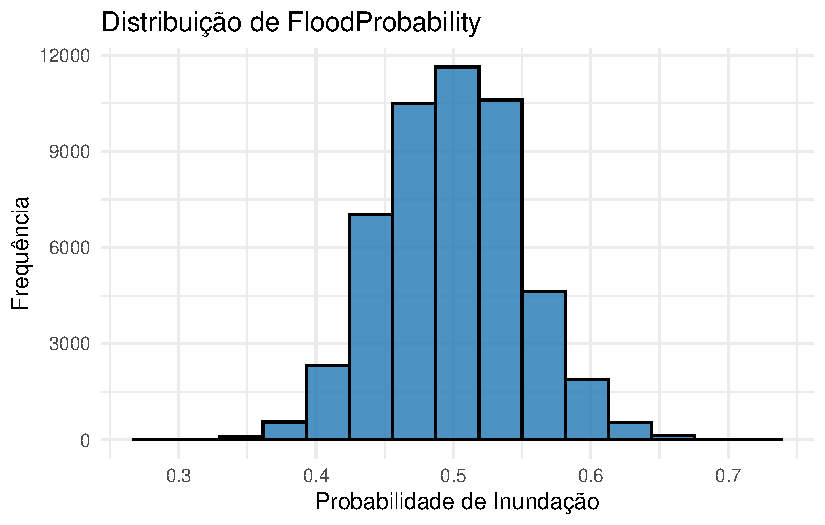
\includegraphics[keepaspectratio]{Flood_Sentinel_files/figure-pdf/unnamed-chunk-9-1.pdf}}

\begin{Shaded}
\begin{Highlighting}[]
\FunctionTok{ggplot}\NormalTok{(df, }\FunctionTok{aes}\NormalTok{(}\AttributeTok{y =}\NormalTok{ FloodProbability)) }\SpecialCharTok{+}
  \FunctionTok{geom\_boxplot}\NormalTok{(}\AttributeTok{fill =} \StringTok{"\#1f77b4"}\NormalTok{, }\AttributeTok{alpha =} \FloatTok{0.6}\NormalTok{) }\SpecialCharTok{+}
  \FunctionTok{labs}\NormalTok{(}
    \AttributeTok{title =} \StringTok{"Boxplot de FloodProbability"}\NormalTok{,}
    \AttributeTok{y =} \StringTok{"Probabilidade de Inundação"}
\NormalTok{  ) }\SpecialCharTok{+}
  \FunctionTok{theme\_minimal}\NormalTok{()}
\end{Highlighting}
\end{Shaded}

\pandocbounded{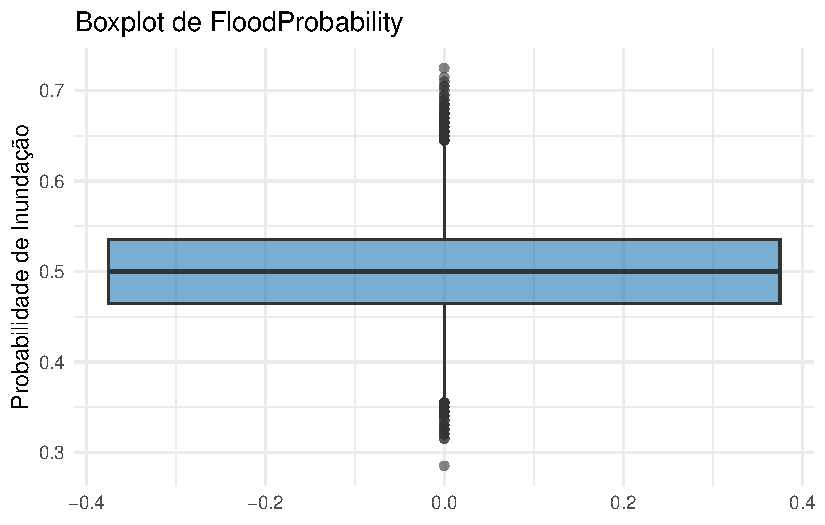
\includegraphics[keepaspectratio]{Flood_Sentinel_files/figure-pdf/unnamed-chunk-9-2.pdf}}

Distribuição das demais variáveis preditoras

\begin{Shaded}
\begin{Highlighting}[]
\FunctionTok{library}\NormalTok{(gridExtra)}
\end{Highlighting}
\end{Shaded}

\begin{verbatim}

Attaching package: 'gridExtra'
\end{verbatim}

\begin{verbatim}
The following object is masked from 'package:dplyr':

    combine
\end{verbatim}

\begin{Shaded}
\begin{Highlighting}[]
\NormalTok{variaveis\_preditoras }\OtherTok{\textless{}{-}}\NormalTok{ df }\SpecialCharTok{\%\textgreater{}\%} \FunctionTok{select}\NormalTok{(}\SpecialCharTok{{-}}\NormalTok{FloodProbability)}


\NormalTok{vars\_to\_plot }\OtherTok{\textless{}{-}} \FunctionTok{names}\NormalTok{(variaveis\_preditoras)[}\DecValTok{1}\SpecialCharTok{:}\DecValTok{4}\NormalTok{]}

\NormalTok{plot\_list }\OtherTok{\textless{}{-}} \FunctionTok{list}\NormalTok{()}
\ControlFlowTok{for}\NormalTok{ (v }\ControlFlowTok{in}\NormalTok{ vars\_to\_plot) \{}
\NormalTok{  p }\OtherTok{\textless{}{-}} \FunctionTok{ggplot}\NormalTok{(df, }\FunctionTok{aes\_string}\NormalTok{(}\AttributeTok{x =}\NormalTok{ v)) }\SpecialCharTok{+}
       \FunctionTok{geom\_histogram}\NormalTok{(}\AttributeTok{bins =} \DecValTok{15}\NormalTok{, }\AttributeTok{fill =} \StringTok{"\#ff7f0e"}\NormalTok{, }\AttributeTok{color =} \StringTok{"black"}\NormalTok{, }\AttributeTok{alpha =} \FloatTok{0.7}\NormalTok{) }\SpecialCharTok{+}
       \FunctionTok{labs}\NormalTok{(}
         \AttributeTok{title =} \FunctionTok{paste}\NormalTok{(}\StringTok{"Distribuição de"}\NormalTok{, v),}
         \AttributeTok{x =}\NormalTok{ v,}
         \AttributeTok{y =} \StringTok{"Frequência"}
\NormalTok{       ) }\SpecialCharTok{+}
       \FunctionTok{theme\_minimal}\NormalTok{()}
\NormalTok{  plot\_list[[v]] }\OtherTok{\textless{}{-}}\NormalTok{ p}
\NormalTok{\}}
\end{Highlighting}
\end{Shaded}

\begin{verbatim}
Warning: `aes_string()` was deprecated in ggplot2 3.0.0.
i Please use tidy evaluation idioms with `aes()`.
i See also `vignette("ggplot2-in-packages")` for more information.
\end{verbatim}

\begin{Shaded}
\begin{Highlighting}[]
\FunctionTok{do.call}\NormalTok{(grid.arrange, }\FunctionTok{c}\NormalTok{(plot\_list, }\AttributeTok{ncol =} \DecValTok{2}\NormalTok{))}
\end{Highlighting}
\end{Shaded}

\pandocbounded{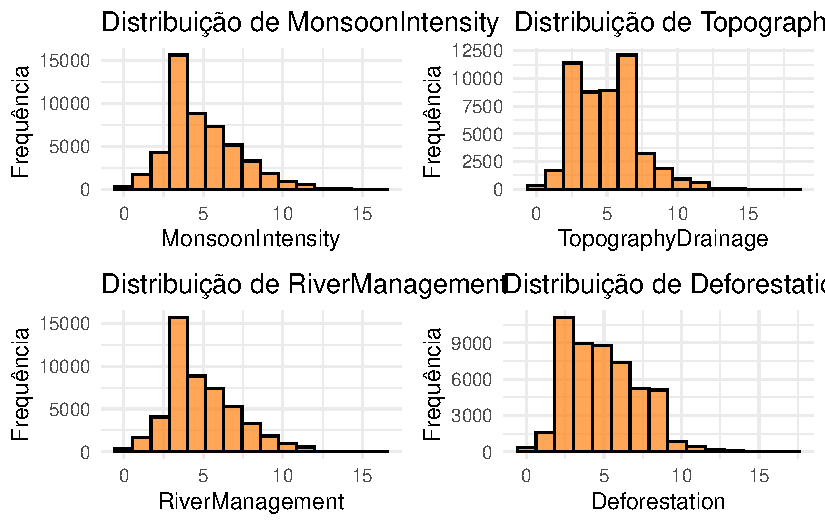
\includegraphics[keepaspectratio]{Flood_Sentinel_files/figure-pdf/unnamed-chunk-10-1.pdf}}

Matriz de Correlação

\begin{Shaded}
\begin{Highlighting}[]
\NormalTok{num\_df }\OtherTok{\textless{}{-}}\NormalTok{ df }\SpecialCharTok{\%\textgreater{}\%} \FunctionTok{select\_if}\NormalTok{(is.numeric)}
\NormalTok{corr\_mat }\OtherTok{\textless{}{-}} \FunctionTok{cor}\NormalTok{(num\_df, }\AttributeTok{use =} \StringTok{"pairwise.complete.obs"}\NormalTok{)}
\end{Highlighting}
\end{Shaded}

Exibir matriz de correlação numérica

\begin{Shaded}
\begin{Highlighting}[]
\FunctionTok{cat}\NormalTok{(}\StringTok{"}\SpecialCharTok{\textbackslash{}n}\StringTok{Matriz de Correlação (primeiras 6 linhas):}\SpecialCharTok{\textbackslash{}n}\StringTok{"}\NormalTok{)}
\end{Highlighting}
\end{Shaded}

\begin{verbatim}

Matriz de Correlação (primeiras 6 linhas):
\end{verbatim}

\begin{Shaded}
\begin{Highlighting}[]
\FunctionTok{print}\NormalTok{(}\FunctionTok{round}\NormalTok{(corr\_mat[}\DecValTok{1}\SpecialCharTok{:}\DecValTok{6}\NormalTok{, }\DecValTok{1}\SpecialCharTok{:}\DecValTok{6}\NormalTok{], }\DecValTok{2}\NormalTok{))}
\end{Highlighting}
\end{Shaded}

\begin{verbatim}
                   MonsoonIntensity TopographyDrainage RiverManagement
MonsoonIntensity               1.00                  0            0.00
TopographyDrainage             0.00                  1            0.00
RiverManagement                0.00                  0            1.00
Deforestation                 -0.01                  0            0.00
Urbanization                   0.01                  0           -0.01
ClimateChange                  0.01                  0            0.01
                   Deforestation Urbanization ClimateChange
MonsoonIntensity           -0.01         0.01          0.01
TopographyDrainage          0.00         0.00          0.00
RiverManagement             0.00        -0.01          0.01
Deforestation               1.00        -0.01          0.00
Urbanization               -0.01         1.00          0.01
ClimateChange               0.00         0.01          1.00
\end{verbatim}

Correlograma completo

\begin{Shaded}
\begin{Highlighting}[]
\FunctionTok{corrplot}\NormalTok{(}
\NormalTok{  corr\_mat,}
  \AttributeTok{method =} \StringTok{"color"}\NormalTok{,}
  \AttributeTok{order =} \StringTok{"hclust"}\NormalTok{,}
  \AttributeTok{tl.cex =} \FloatTok{0.7}\NormalTok{,}
  \AttributeTok{addCoef.col =} \StringTok{"black"}\NormalTok{,}
  \AttributeTok{number.cex =} \FloatTok{0.6}\NormalTok{,}
  \AttributeTok{tl.col =} \StringTok{"black"}\NormalTok{,}
  \AttributeTok{col =} \FunctionTok{colorRampPalette}\NormalTok{(}\FunctionTok{c}\NormalTok{(}\StringTok{"blue"}\NormalTok{, }\StringTok{"white"}\NormalTok{, }\StringTok{"red"}\NormalTok{))(}\DecValTok{200}\NormalTok{),}
  \AttributeTok{title =} \StringTok{"Correlograma das Variáveis"}
\NormalTok{)}
\end{Highlighting}
\end{Shaded}

\pandocbounded{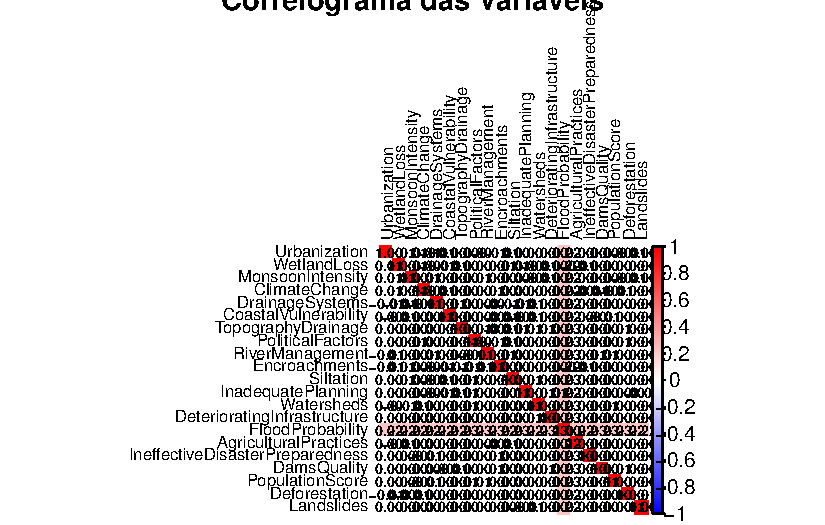
\includegraphics[keepaspectratio]{Flood_Sentinel_files/figure-pdf/unnamed-chunk-13-1.pdf}}

Pair Plot (GGally) para subconjunto de variáveis

\begin{Shaded}
\begin{Highlighting}[]
\NormalTok{corr\_flood }\OtherTok{\textless{}{-}}\NormalTok{ corr\_mat[, }\StringTok{"FloodProbability"}\NormalTok{] }\SpecialCharTok{\%\textgreater{}\%}
  \FunctionTok{abs}\NormalTok{() }\SpecialCharTok{\%\textgreater{}\%}
  \FunctionTok{sort}\NormalTok{(}\AttributeTok{decreasing =} \ConstantTok{TRUE}\NormalTok{)}
\NormalTok{top\_pred }\OtherTok{\textless{}{-}} \FunctionTok{names}\NormalTok{(corr\_flood)[}\DecValTok{2}\SpecialCharTok{:}\DecValTok{5}\NormalTok{]}
\NormalTok{pair\_df }\OtherTok{\textless{}{-}}\NormalTok{ df }\SpecialCharTok{\%\textgreater{}\%} \FunctionTok{select}\NormalTok{(}\FunctionTok{all\_of}\NormalTok{(}\FunctionTok{c}\NormalTok{(}\StringTok{"FloodProbability"}\NormalTok{, top\_pred)))}

\FunctionTok{ggpairs}\NormalTok{(}
\NormalTok{  pair\_df,}
  \AttributeTok{upper =} \FunctionTok{list}\NormalTok{(}\AttributeTok{continuous =} \FunctionTok{wrap}\NormalTok{(}\StringTok{"points"}\NormalTok{, }\AttributeTok{alpha =} \FloatTok{0.4}\NormalTok{, }\AttributeTok{size =} \FloatTok{0.8}\NormalTok{)),}
  \AttributeTok{lower =} \FunctionTok{list}\NormalTok{(}\AttributeTok{continuous =} \FunctionTok{wrap}\NormalTok{(}\StringTok{"smooth"}\NormalTok{, }\AttributeTok{se =} \ConstantTok{FALSE}\NormalTok{, }\AttributeTok{alpha =} \FloatTok{0.3}\NormalTok{)),}
  \AttributeTok{diag =} \FunctionTok{list}\NormalTok{(}\AttributeTok{continuous =} \FunctionTok{wrap}\NormalTok{(}\StringTok{"densityDiag"}\NormalTok{)),}
  \AttributeTok{title =} \StringTok{"Pair Plot entre FloodProbability e as 4 variáveis mais correlacionadas"}
\NormalTok{)}
\end{Highlighting}
\end{Shaded}

\pandocbounded{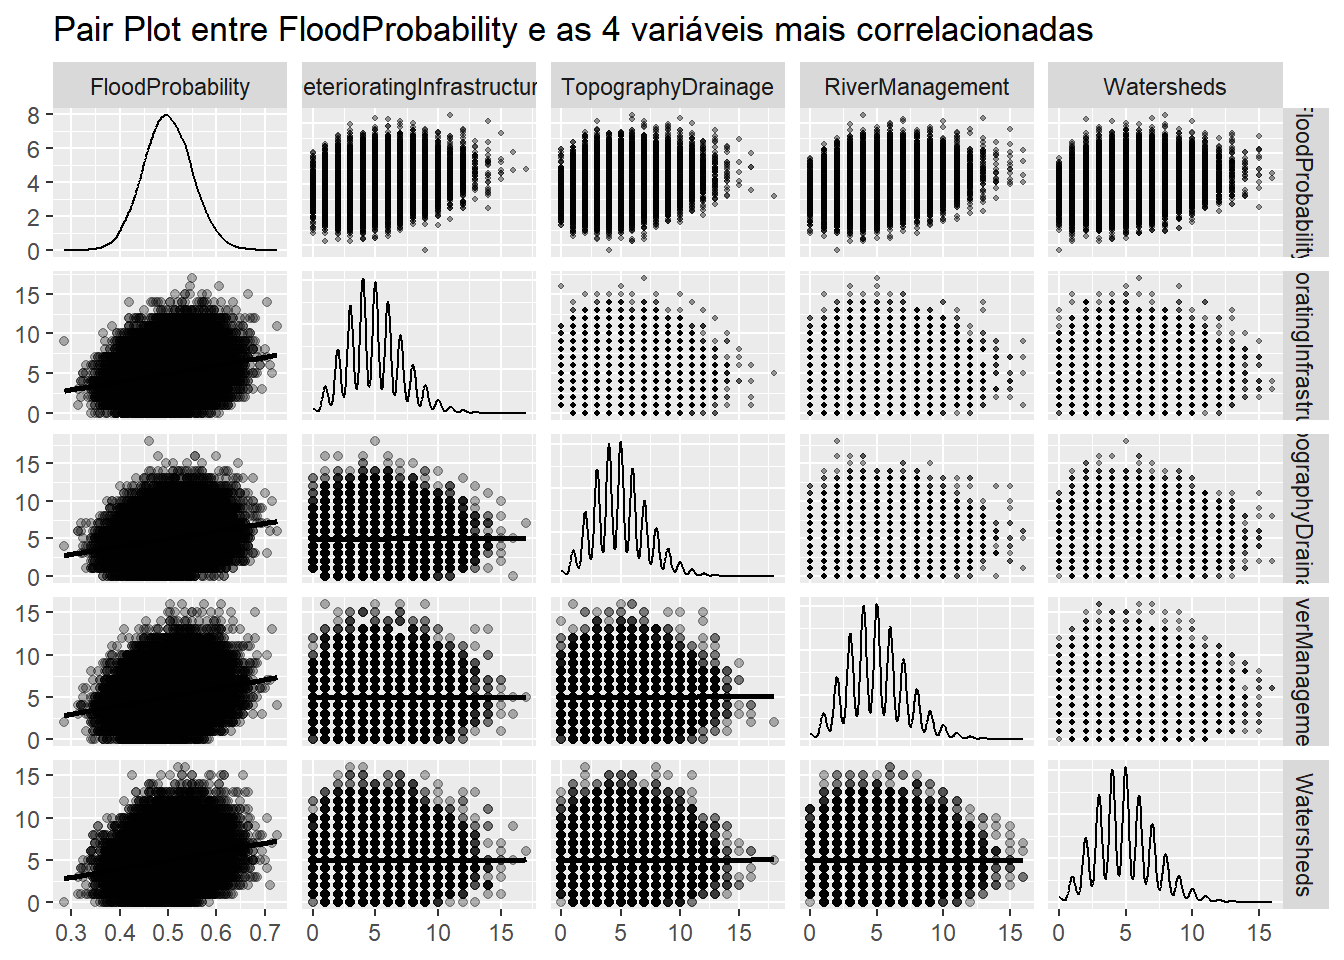
\includegraphics[keepaspectratio]{Flood_Sentinel_files/figure-pdf/unnamed-chunk-14-1.pdf}}

\subsection{Análise Explanatória}\label{anuxe1lise-explanatuxf3ria}

separar variaveis de teste:

\begin{Shaded}
\begin{Highlighting}[]
\FunctionTok{set.seed}\NormalTok{(}\DecValTok{123}\NormalTok{)}
\NormalTok{train\_indices }\OtherTok{\textless{}{-}} \FunctionTok{sample}\NormalTok{(}\FunctionTok{seq\_len}\NormalTok{(}\FunctionTok{nrow}\NormalTok{(df)), }\AttributeTok{size =} \FloatTok{0.7} \SpecialCharTok{*} \FunctionTok{nrow}\NormalTok{(df))}
\NormalTok{df\_train }\OtherTok{\textless{}{-}}\NormalTok{ df[train\_indices, ]}
\NormalTok{df\_test  }\OtherTok{\textless{}{-}}\NormalTok{ df[}\SpecialCharTok{{-}}\NormalTok{train\_indices, ]}
\end{Highlighting}
\end{Shaded}

Modelo de Regressão Linear Múltipla

Selecionamos as 5 variáveis de maior correlação (absoluta) com
FloodProbability

\begin{Shaded}
\begin{Highlighting}[]
\NormalTok{top5\_vars }\OtherTok{\textless{}{-}} \FunctionTok{names}\NormalTok{(corr\_flood)[}\DecValTok{2}\SpecialCharTok{:}\DecValTok{6}\NormalTok{] }

\FunctionTok{cat}\NormalTok{(}\StringTok{"}\SpecialCharTok{\textbackslash{}n}\StringTok{Variáveis selecionadas para o modelo:"}\NormalTok{, }\FunctionTok{paste}\NormalTok{(top5\_vars, }\AttributeTok{collapse =} \StringTok{", "}\NormalTok{), }\StringTok{"}\SpecialCharTok{\textbackslash{}n}\StringTok{"}\NormalTok{)}
\end{Highlighting}
\end{Shaded}

\begin{verbatim}

Variáveis selecionadas para o modelo: DeterioratingInfrastructure, TopographyDrainage, RiverManagement, Watersheds, DamsQuality 
\end{verbatim}

\begin{Shaded}
\begin{Highlighting}[]
\NormalTok{formula\_modelo }\OtherTok{\textless{}{-}} \FunctionTok{as.formula}\NormalTok{(}
  \FunctionTok{paste}\NormalTok{(}\StringTok{"FloodProbability \textasciitilde{}"}\NormalTok{, }\FunctionTok{paste}\NormalTok{(top5\_vars, }\AttributeTok{collapse =} \StringTok{" + "}\NormalTok{))}
\NormalTok{)}
\end{Highlighting}
\end{Shaded}

\begin{Shaded}
\begin{Highlighting}[]
\NormalTok{modelo\_lm }\OtherTok{\textless{}{-}} \FunctionTok{lm}\NormalTok{(formula\_modelo, }\AttributeTok{data =}\NormalTok{ df\_train)}
\FunctionTok{cat}\NormalTok{(}\StringTok{"}\SpecialCharTok{\textbackslash{}n}\StringTok{Resumo do modelo de Regressão Linear:}\SpecialCharTok{\textbackslash{}n}\StringTok{"}\NormalTok{)}
\end{Highlighting}
\end{Shaded}

\begin{verbatim}

Resumo do modelo de Regressão Linear:
\end{verbatim}

\begin{Shaded}
\begin{Highlighting}[]
\FunctionTok{print}\NormalTok{(}\FunctionTok{summary}\NormalTok{(modelo\_lm))}
\end{Highlighting}
\end{Shaded}

\begin{verbatim}

Call:
lm(formula = formula_modelo, data = df_train)

Residuals:
      Min        1Q    Median        3Q       Max 
-0.174075 -0.029604  0.000009  0.029810  0.189549 

Coefficients:
                             Estimate Std. Error t value Pr(>|t|)    
(Intercept)                 0.3726657  0.0011726  317.81   <2e-16 ***
DeterioratingInfrastructure 0.0050384  0.0001036   48.62   <2e-16 ***
TopographyDrainage          0.0051573  0.0001027   50.22   <2e-16 ***
RiverManagement             0.0050900  0.0001034   49.23   <2e-16 ***
Watersheds                  0.0049815  0.0001033   48.23   <2e-16 ***
DamsQuality                 0.0051272  0.0001029   49.83   <2e-16 ***
---
Signif. codes:  0 '***' 0.001 '**' 0.01 '*' 0.05 '.' 0.1 ' ' 1

Residual standard error: 0.04319 on 34994 degrees of freedom
Multiple R-squared:  0.258, Adjusted R-squared:  0.2579 
F-statistic:  2434 on 5 and 34994 DF,  p-value: < 2.2e-16
\end{verbatim}

Avaliar suposições: resíduos vs valores ajustados

\begin{Shaded}
\begin{Highlighting}[]
\FunctionTok{par}\NormalTok{(}\AttributeTok{mfrow =} \FunctionTok{c}\NormalTok{(}\DecValTok{2}\NormalTok{, }\DecValTok{2}\NormalTok{))}
\FunctionTok{plot}\NormalTok{(modelo\_lm)}
\end{Highlighting}
\end{Shaded}

\pandocbounded{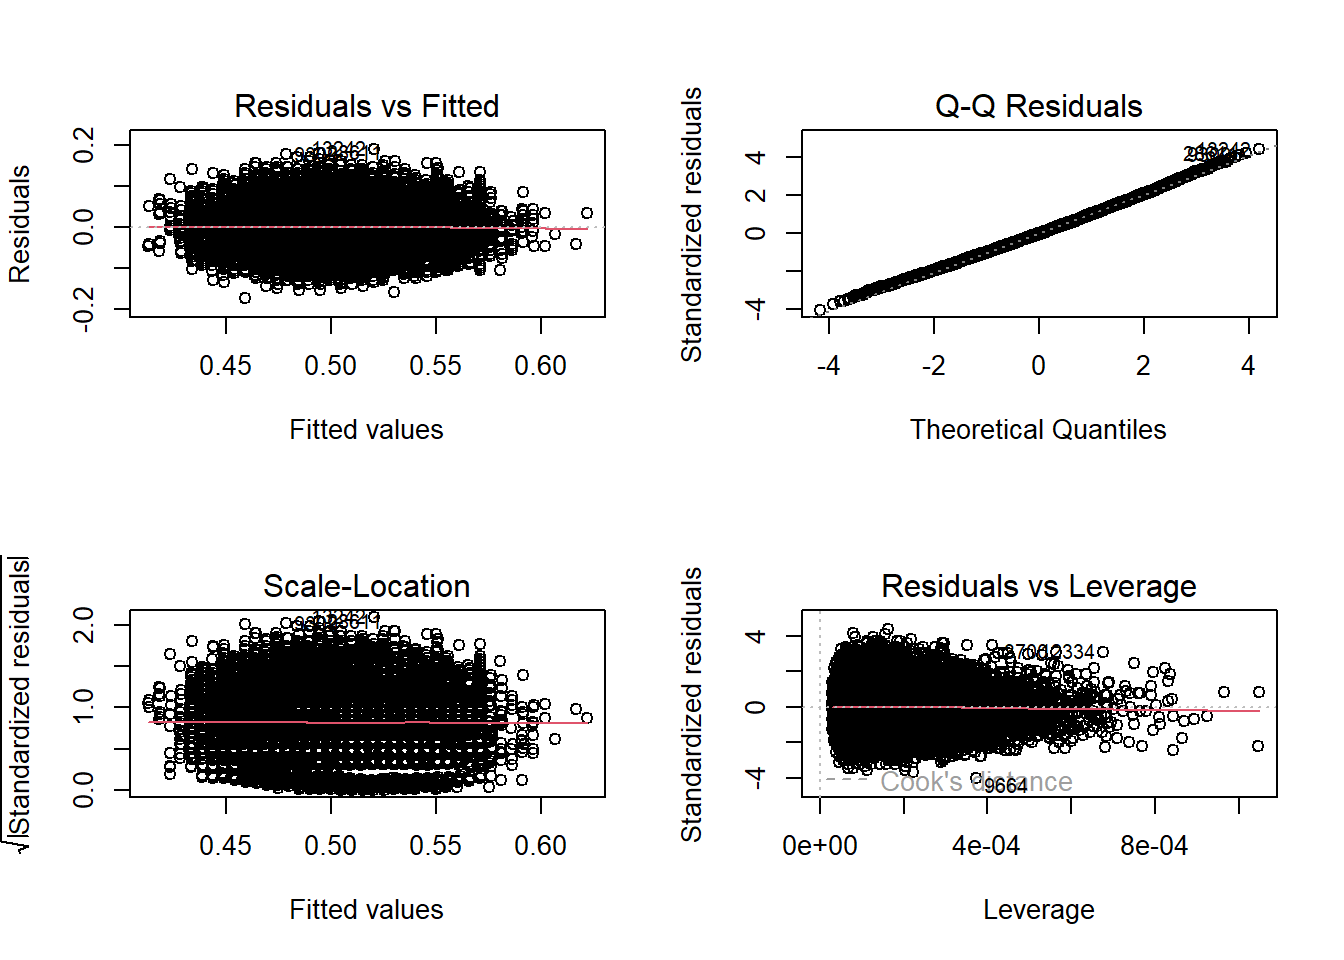
\includegraphics[keepaspectratio]{Flood_Sentinel_files/figure-pdf/unnamed-chunk-19-1.pdf}}

\begin{Shaded}
\begin{Highlighting}[]
\FunctionTok{par}\NormalTok{(}\AttributeTok{mfrow =} \FunctionTok{c}\NormalTok{(}\DecValTok{1}\NormalTok{, }\DecValTok{1}\NormalTok{))}
\end{Highlighting}
\end{Shaded}

Previsão e Métricas no Conjunto de Teste

\begin{Shaded}
\begin{Highlighting}[]
\NormalTok{pred\_test }\OtherTok{\textless{}{-}} \FunctionTok{predict}\NormalTok{(modelo\_lm, }\AttributeTok{newdata =}\NormalTok{ df\_test)}

\FunctionTok{library}\NormalTok{(Metrics)  }\CommentTok{\# para RMSE e MAE}
\NormalTok{rmse\_val  }\OtherTok{\textless{}{-}} \FunctionTok{rmse}\NormalTok{(df\_test}\SpecialCharTok{$}\NormalTok{FloodProbability, pred\_test)}
\NormalTok{mae\_val   }\OtherTok{\textless{}{-}} \FunctionTok{mae}\NormalTok{(df\_test}\SpecialCharTok{$}\NormalTok{FloodProbability, pred\_test)}
\NormalTok{mape\_val  }\OtherTok{\textless{}{-}} \FunctionTok{mape}\NormalTok{(df\_test}\SpecialCharTok{$}\NormalTok{FloodProbability, pred\_test) }\SpecialCharTok{*} \DecValTok{100}

\FunctionTok{cat}\NormalTok{(}\FunctionTok{sprintf}\NormalTok{(}\StringTok{"}\SpecialCharTok{\textbackslash{}n}\StringTok{Métricas no conjunto de teste:}\SpecialCharTok{\textbackslash{}n}\StringTok{  RMSE = \%.4f}\SpecialCharTok{\textbackslash{}n}\StringTok{  MAE  = \%.4f}\SpecialCharTok{\textbackslash{}n}\StringTok{  MAPE = \%.2f\%\%}\SpecialCharTok{\textbackslash{}n}\StringTok{"}\NormalTok{,}
\NormalTok{            rmse\_val, mae\_val, mape\_val))}
\end{Highlighting}
\end{Shaded}

\begin{verbatim}

Métricas no conjunto de teste:
  RMSE = 0.0428
  MAE  = 0.0341
  MAPE = 6.92%
\end{verbatim}

Gráfico de Previsão vs Observado

\begin{Shaded}
\begin{Highlighting}[]
\NormalTok{df\_pred\_obs }\OtherTok{\textless{}{-}} \FunctionTok{tibble}\NormalTok{(}
  \AttributeTok{Observado  =}\NormalTok{ df\_test}\SpecialCharTok{$}\NormalTok{FloodProbability,}
  \AttributeTok{Previsto   =}\NormalTok{ pred\_test}
\NormalTok{)}

\FunctionTok{ggplot}\NormalTok{(df\_pred\_obs, }\FunctionTok{aes}\NormalTok{(}\AttributeTok{x =}\NormalTok{ Observado, }\AttributeTok{y =}\NormalTok{ Previsto)) }\SpecialCharTok{+}
  \FunctionTok{geom\_point}\NormalTok{(}\AttributeTok{alpha =} \FloatTok{0.6}\NormalTok{, }\AttributeTok{color =} \StringTok{"\#2ca02c"}\NormalTok{) }\SpecialCharTok{+}
  \FunctionTok{geom\_abline}\NormalTok{(}\AttributeTok{slope =} \DecValTok{1}\NormalTok{, }\AttributeTok{intercept =} \DecValTok{0}\NormalTok{, }\AttributeTok{linetype =} \StringTok{"dashed"}\NormalTok{, }\AttributeTok{color =} \StringTok{"red"}\NormalTok{) }\SpecialCharTok{+}
  \FunctionTok{labs}\NormalTok{(}
    \AttributeTok{title =} \StringTok{"Observado vs Previsto (Conjunto de Teste)"}\NormalTok{,}
    \AttributeTok{x =} \StringTok{"FloodProbability Observado"}\NormalTok{,}
    \AttributeTok{y =} \StringTok{"FloodProbability Previsto"}
\NormalTok{  ) }\SpecialCharTok{+}
  \FunctionTok{theme\_minimal}\NormalTok{()}
\end{Highlighting}
\end{Shaded}

\pandocbounded{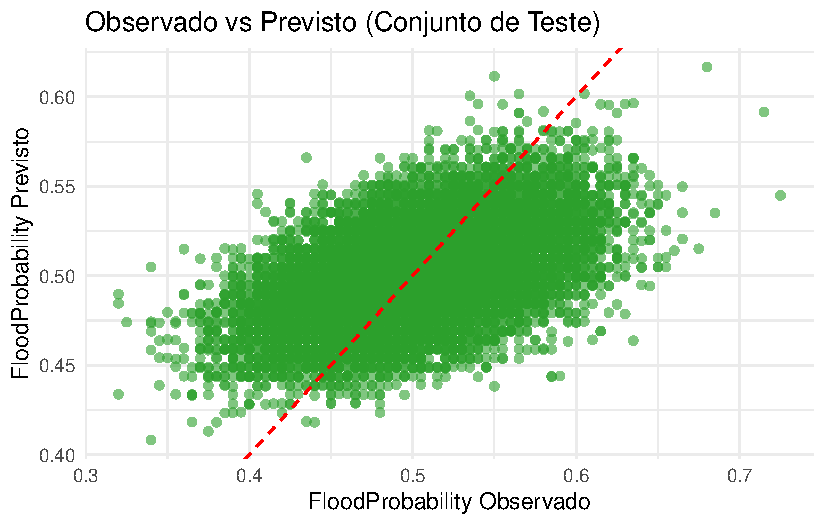
\includegraphics[keepaspectratio]{Flood_Sentinel_files/figure-pdf/unnamed-chunk-21-1.pdf}}

Interpretação dos Resultados

\begin{Shaded}
\begin{Highlighting}[]
\FunctionTok{cat}\NormalTok{(}\StringTok{"}\SpecialCharTok{\textbackslash{}n}\StringTok{Coeficientes do modelo:}\SpecialCharTok{\textbackslash{}n}\StringTok{"}\NormalTok{)}
\end{Highlighting}
\end{Shaded}

\begin{verbatim}

Coeficientes do modelo:
\end{verbatim}

\begin{Shaded}
\begin{Highlighting}[]
\NormalTok{coef\_df }\OtherTok{\textless{}{-}}\NormalTok{ broom}\SpecialCharTok{::}\FunctionTok{tidy}\NormalTok{(modelo\_lm)}
\FunctionTok{kable}\NormalTok{(coef\_df, }\AttributeTok{digits =} \DecValTok{4}\NormalTok{, }\AttributeTok{col.names =} \FunctionTok{c}\NormalTok{(}\StringTok{"Termo"}\NormalTok{, }\StringTok{"Estimativa"}\NormalTok{, }\StringTok{"Std. Erro"}\NormalTok{, }\StringTok{"t valor"}\NormalTok{, }\StringTok{"Pr(\textgreater{}|t|)"}\NormalTok{))}
\end{Highlighting}
\end{Shaded}

\begin{longtable}[]{@{}
  >{\raggedright\arraybackslash}p{(\linewidth - 8\tabcolsep) * \real{0.3636}}
  >{\raggedleft\arraybackslash}p{(\linewidth - 8\tabcolsep) * \real{0.1429}}
  >{\raggedleft\arraybackslash}p{(\linewidth - 8\tabcolsep) * \real{0.1299}}
  >{\raggedleft\arraybackslash}p{(\linewidth - 8\tabcolsep) * \real{0.1169}}
  >{\raggedleft\arraybackslash}p{(\linewidth - 8\tabcolsep) * \real{0.2468}}@{}}
\toprule\noalign{}
\begin{minipage}[b]{\linewidth}\raggedright
Termo
\end{minipage} & \begin{minipage}[b]{\linewidth}\raggedleft
Estimativa
\end{minipage} & \begin{minipage}[b]{\linewidth}\raggedleft
Std. Erro
\end{minipage} & \begin{minipage}[b]{\linewidth}\raggedleft
t valor
\end{minipage} & \begin{minipage}[b]{\linewidth}\raggedleft
Pr(\textgreater\textbar t\textbar)
\end{minipage} \\
\midrule\noalign{}
\endhead
\bottomrule\noalign{}
\endlastfoot
(Intercept) & 0.3727 & 0.0012 & 317.8149 & 0 \\
DeterioratingInfrastructure & 0.0050 & 0.0001 & 48.6168 & 0 \\
TopographyDrainage & 0.0052 & 0.0001 & 50.2181 & 0 \\
RiverManagement & 0.0051 & 0.0001 & 49.2267 & 0 \\
Watersheds & 0.0050 & 0.0001 & 48.2252 & 0 \\
DamsQuality & 0.0051 & 0.0001 & 49.8323 & 0 \\
\end{longtable}

\begin{Shaded}
\begin{Highlighting}[]
\FunctionTok{cat}\NormalTok{(}\StringTok{"}\SpecialCharTok{\textbackslash{}n}\StringTok{Interpretação resumida:}\SpecialCharTok{\textbackslash{}n}\StringTok{"}\NormalTok{)}
\end{Highlighting}
\end{Shaded}

\begin{verbatim}

Interpretação resumida:
\end{verbatim}

\begin{Shaded}
\begin{Highlighting}[]
\FunctionTok{cat}\NormalTok{(}\StringTok{"}
\StringTok{{-} O modelo de regressão explica aproximadamente"}\NormalTok{, }\FunctionTok{round}\NormalTok{(}\FunctionTok{summary}\NormalTok{(modelo\_lm)}\SpecialCharTok{$}\NormalTok{r.squared, }\DecValTok{3}\NormalTok{),}
    \StringTok{"dos desvios em FloodProbability (R² ajustado ="}\NormalTok{,}
    \FunctionTok{round}\NormalTok{(}\FunctionTok{summary}\NormalTok{(modelo\_lm)}\SpecialCharTok{$}\NormalTok{adj.r.squared, }\DecValTok{3}\NormalTok{), }\StringTok{").}\SpecialCharTok{\textbackslash{}n}
\StringTok{{-} Variáveis com p{-}valor \textless{} 0.05 indicam influência estatisticamente significativa sobre FloodProbability.}
\StringTok{{-} Os coeficientes positivos (p.ex., se \textquotesingle{}DeterioratingInfrastructure\textquotesingle{} tiver coeff \textgreater{} 0) sugerem que,}
\StringTok{  para cada unidade adicional nessa variável, a probabilidade de inundação tende a aumentar, mantidas as demais constantes.}
\StringTok{{-} Da mesma forma, coeficientes negativos indicam relação inversa.}\SpecialCharTok{\textbackslash{}n}
\StringTok{{-} As métricas de erro no conjunto de teste (RMSE ="}\NormalTok{, }\FunctionTok{round}\NormalTok{(rmse\_val, }\DecValTok{4}\NormalTok{),}
    \StringTok{", MAE ="}\NormalTok{, }\FunctionTok{round}\NormalTok{(mae\_val, }\DecValTok{4}\NormalTok{), }\StringTok{", MAPE ="}\NormalTok{, }\FunctionTok{round}\NormalTok{(mape\_val, }\DecValTok{2}\NormalTok{), }\StringTok{"\%) fornecem feedback sobre o quão bem o modelo está prevendo.}\SpecialCharTok{\textbackslash{}n}
\StringTok{{-} Gráfico Observado vs Previsto: se a maioria dos pontos estiver próxima à linha pontilhada (y = x), o modelo tem bom desempenho.}\SpecialCharTok{\textbackslash{}n}
\StringTok{"}\NormalTok{)}
\end{Highlighting}
\end{Shaded}

\begin{verbatim}

- O modelo de regressão explica aproximadamente 0.258 dos desvios em FloodProbability (R² ajustado = 0.258 ).

- Variáveis com p-valor < 0.05 indicam influência estatisticamente significativa sobre FloodProbability.
- Os coeficientes positivos (p.ex., se 'DeterioratingInfrastructure' tiver coeff > 0) sugerem que,
  para cada unidade adicional nessa variável, a probabilidade de inundação tende a aumentar, mantidas as demais constantes.
- Da mesma forma, coeficientes negativos indicam relação inversa.

- As métricas de erro no conjunto de teste (RMSE = 0.0428 , MAE = 0.0341 , MAPE = 6.92 %) fornecem feedback sobre o quão bem o modelo está prevendo.

- Gráfico Observado vs Previsto: se a maioria dos pontos estiver próxima à linha pontilhada (y = x), o modelo tem bom desempenho.
\end{verbatim}




\end{document}
